\chapter{NoSQL}
\begin{nota}
    In quest capitolo non si vuole sostenere che i database NoSQL siano
    migliori di quelli relazionali. I database NoSQL sono un'alternativa
    ai database relazionali e non sempre sono la scelta migliore. Per ogni
    applicazione è necessario valutare quale sia la scelta migliore.
\end{nota}
Fino a questo momento abbiamo utilizzato database relazionali per gestire le
nostre applicazioni. Tuttavia, i database relazionali non sono l'unica
opzione disponibile. In questo capitolo, esploreremo un'alternativa ai
database relazionali: i database NoSQL.
\section*{Use Cases}
\subsection*{Crypto}
Iniziamo analizzando uno Use Case. Un cliente vuole salvare dati legati alle
crypto che vengono forniti da un API. Con le conoscenze conseguite fino a questo
momento, salveremo tutto su una tabella di un DBMS relazionale dove si hanno 5 colonne:
\begin{itemize}
    \item id
    \item Simbolo
    \item Prezzo\_USD
    \item Prezzo\_EUR
    \item Data
\end{itemize}
Nel caso in cui nella risposta fossero presenti informazioni aggiuntive o nel caso
in cui si volessero salvare informazioni aggiuntive, si dovrebbe modificare la
tabella. Questo si può osservare soprattutto quando si hanno risposte molto
complesse, perché salvare dati in molteplici tabelle significa per ottenere
l'informazione intera si devono fare molte join, questo comporta un rallentamento
delle prestazioni.

Una soluzione per ridurre il numero di join è quello di duplicare i dati, il
problema è che i dati che si duplicano devono essere consistenti. In aggiunta
posso ridurre le tabelle unendole creando una grande tabella che può essere
frammentata a livello fisico, il problema di questa soluzione è che si vanno a
inserire un elevato numero di valori \texttt{null}.
\subsection*{Social network}
Un altro caso d'uso è il social network in cui si vuole salvare la relazione di
amicizia tra profili, il problema è che se si avessero 1M di utenti, ciascuno con
100 amici, allora la tabella amicizia diventa 100M di record. Troppa complessità
soprattutto per una tabella che verrà usata spesso con delle join.

Il DB relazionali non sono in grado di modellare efficientemente i contesti applicativi
con volumi molto significativi di dati.
\section{Introduzione}
Da questo use case possiamo osservare che il modello relazionale presenta dei
limiti nella gestione dei dati:
\begin{itemize}
    \item Si ha uno svantaggio nel salvare di dati poco omogenei, questo è dovuto
          principalmente alla rigidità dello schema. In quanto prima di poter
          inserire i dati, è necessario definire uno schema.
    \item Si ha uno svantaggio in relazione al paradigma di programmazione che
          viene usato (Programmazione a oggetti). Questo obbliga a utilizzare
          un ORM per mappare i dati del database relazionale con gli oggetti
          del linguaggio di programmazione.
\end{itemize}
Inoltre, essendo le risposte delle API solitamente in formato JSON, si ha un
ulteriore svantaggio in quanto si deve fare un parsing della risposta per
poterla salvare nel database relazionale.

I database NoSQL sono nati con lo scopo di risolvere alcuni problemi di quelli
relazionali come la scalabilità e la flessibilità. Inoltre, le assunzioni che
si trovano dietro i database relazionali non sono sempre adatte per tutti i
casi d'uso.

Con questo non vogliamo dire che i database NoSQL siano migliori di quelli
relazionali, ma che sono un'alternativa ai database relazionali. Per ogni
applicazione è necessario valutare quale sia la scelta migliore. Di seguito
elenchiamo alcuni motivi per cui utilizzare i database relazionali:
\begin{itemize}
    \item SQL è semplice.
    \item Molto rigido
    \item Vincoli nel database allora le app possono non fare i controlli
    \item ipotesi di mondo chiuso: tutto quello che serve è nel database, se non
          lo so devo inserire il valore \texttt{null}.
    \item Tecnologia stabile e funzionante che alle spalle anni di ricerca e
          sviluppo.
    \item Sono valide le proprietà ACID, molto utili in contesti in cui si
          hanno transazioni.
\end{itemize}
È corretto presentare anche gli svantaggi dei database relazionali:
\begin{itemize}
    \item Modificare una tabella nella quale sono già presenti dei valori è molto
          complicato.
    \item Assunzione mondo chiuso: può risultare troppo pesante in determinate
          situazioni.
    \item Il concetto di minimizzare le ripetizioni dei valori implica la necessità
          di effettuare molte join per ottenere l'informazione desiderata.
    \item Si ha un mapping un attributo ha un valore.
    \item Non è compatibile con i linguaggi di programmazione ad oggetti.
    \item Presenta delle difficoltà nella gestione dei self-join.
    \item È difficilmente scalabile.
\end{itemize}
\begin{nota}
    Il termine NoSQL significa \textit{Not Only SQL}.
\end{nota}
Una caratteristica comune dei database NoSQL è che sono \textbf{schema-free} o
\textbf{schema-less}. Questo significa che non è necessario definire uno schema
prima di poter inserire i dati. L'inserimento dei dati implica per quel dato lo
schema associato, il successivo inserimento di un dato può avere uno schema diverso.

% Presa da internet la definizione
Oltre a ciò, per questi database vale il teorema CAP, che afferma che è
impossibile per un sistema distribuito garantire contemporaneamente le seguenti
tre proprietà:
\begin{itemize}
    \item \textbf{Consistency}: tutti i nodi vedono gli stessi dati allo stesso
          tempo.
    \item \textbf{Availability}: ogni richiesta riceve una risposta, anche in
          presenza di guasti.
    \item \textbf{Partition tolerance}: il sistema continua a funzionare anche
          se alcune parti del sistema non sono disponibili.
\end{itemize}

Mentre nei database relazionali avevamo le transazioni ACID, nei database NoSQL
abbiamo le transazioni BASE, che stanno per:
\begin{itemize}
    \item \textbf{Basically Available}: il sistema è sempre disponibile.
    \item \textbf{Soft state}: lo stato del sistema può cambiare anche senza
          input.
    \item \textbf{Eventual consistency}: il sistema diventerà consistente in un
          certo momento.
\end{itemize}

Inoltre, a differenza dei database relazionali, i database NoSQL si basano su 
un'assunzione di mondo aperto, ovvero viene inserito solo quello che conosco se 
mi mancano delle informazioni non le metto.

Si è passati dal progettare le architetture in modo da essere più specifiche
per l'applicazione, il contrario di come si faceva una volta: progettazione generalista.
\section{Tipi di database NoSQL}
Esistono diverse tipologie di database NoSQL, ognuna con le proprie caratteristiche
e i propri casi d'uso. Possiamo dire che più è semplice il modello, più è facile
scalarlo. Nella figura \ref{fig:tipi_nosql} possiamo come si posizionano i
database NoSQL rispetto alla dimensione e complessità del modello.
\begin{figure}[!ht]
    \centering
    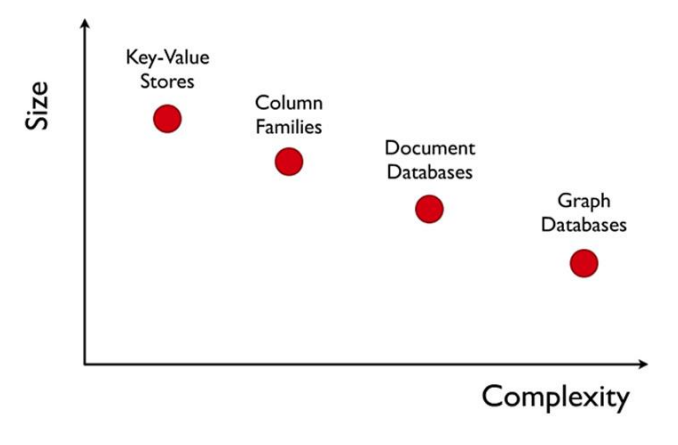
\includegraphics[scale=0.5]{./img/nosql/tipi_nosql.png}
    \caption{Tipi di database NoSQL}
    \label{fig:tipi_nosql}
\end{figure}
Rispetto questa rappresentazione possiamo posizionare il modello relazionale a metà
tra la complessità delle colonne e i documenti.
In questo corso vedremo i seguenti tipi di database NoSQL:
\begin{itemize}
    \item \textbf{Document-based}: i dati sono memorizzati in documenti, che
          possono essere in formato JSON, XML, BSON, YAML, etc.
    \item \textbf{Key-value}: i dati sono memorizzati in coppie chiave-valore.
    \item \textbf{Wide-column}: i dati sono memorizzati in colonne, simile ai
          database relazionali.
    \item \textbf{Graph-based}: i dati sono memorizzati in nodi e archi.
\end{itemize}
Una caratteristica che accomuna questi modelli è che tutti devono risolvere il 
problema di mettere insieme i dati. Ad esempio, i database relazionali usano i join,
mentre i database document-based usano un unico documento.
\subsection{Key value}
I database key-value sono i più semplici tra i database NoSQL. In questi
database, i dati sono memorizzati come tabelle di hash dove la chiave punta a un
particolare valore. Si utilizzano le tabelle di hash per massimizzare le prestazioni
di lettura e scrittura.
\subsection{Wide column}
I database wide-column sono simili ai database relazionali, ma invece di
memorizzare i dati in righe, i dati sono memorizzati in colonne. Questo permette
di avere una maggiore flessibilità rispetto ai database relazionali. La chiave
punta a un insieme di colonne che può essere diverso per ogni riga.
\subsection{Document based}
I database document-based memorizzano i dati in documenti. I documenti sono
indirizzati nel database tramite una chiave unica. La ricerca dei dati è
effettuata nei documenti stessi.
\subsection{Graph based}
I database graph-based memorizzano i dati in nodi e archi. Questi database sono
utili per memorizzare dati che hanno relazioni complesse. I nodi rappresentano
le entità e gli archi rappresentano le relazioni tra le entità.

